\documentclass[12pt,letterpaper,oneside]{report}

\usepackage[T1]{fontenc}
\usepackage[utf8]{inputenc}
\usepackage{lmodern}
\usepackage[margin=1in]{geometry}
\usepackage{setspace}
\usepackage{microtype}
\usepackage{amsmath,amssymb}
\usepackage{graphicx}
\usepackage{booktabs}
\usepackage{array}
\usepackage{enumitem}
\usepackage{xcolor}
\usepackage{csquotes}
\usepackage{hyperref}
\usepackage[nameinlink,noabbrev]{cleveref}

\usepackage[
  backend=biber,
  style=numeric,
  sorting=none,
  maxbibnames=99
]{biblatex}
\addbibresource{references.bib}

\hypersetup{
  colorlinks=true,
  linkcolor=blue!45!black,
  citecolor=green!35!black,
  urlcolor=blue!55!black,
  pdftitle={Numerical variability of functional MRI graph measures},
  pdfauthor={Mina Alizadeh}
}

\graphicspath{{figures/}}
\setlist{nosep}
\onehalfspacing
\setlength{\parskip}{0.35em}
\setlength{\parindent}{1.5em}

\newcommand{\npvr}{\ensuremath{\nu_{\mathrm{npv}}}}
\newcommand{\npvratio}{NPVR}
\newcommand{\projecttitle}{Numerical variability of functional MRI graph measures}

\begin{document}

\hypersetup{pageanchor=false}
\begin{titlepage}
  \centering
  \vspace*{1.25in}
  {\Large\bfseries \projecttitle\par}
  \vspace{0.7in}
  {\large Doctoral Research Proposal (ENCS 8511)\par}
  \vspace{0.25in}
  {\large Mina Alizadeh\par}
  \vfill
  {\large Department of Computer Science and Software Engineering\par}
  {\large Gina Cody School of Engineering and Computer Science\par}
  {\large Concordia University\par}
  \vspace{0.5in}
  {\large Co-supervisors: Tristan Glatard and Gregory Kiar\par}
  \vspace{0.5in}
  {\large \today\par}
\end{titlepage}

\hypersetup{pageanchor=true}
\pagenumbering{roman}
\chapter*{Summary}
\addcontentsline{toc}{chapter}{Summary}
\begin{singlespace}

Resting-state functional magnetic resonance imaging (rs-fMRI) and graph theory offer a non-invasive way to study network-level alterations associated with Parkinson's disease (PD). Their scientific and eventual clinical value, however, depends on results that remain reliable when reasonable analytical choices or computational environments change. 
As analyses become increasingly computational, ensuring their numerical reliability has become a critical challenge. Small perturbations introduced during processing can propagate through complex pipelines, leading to variability in outcomes and raising concerns about the reproducibility of reported findings. Addressing this issue requires systematic evaluation of pipeline stability to ensure results remain within acceptable numerical limits. 

This doctoral research investigates the numerical variability of functional MRI graph measures. The central objective is to systematically evaluate the numerical variability of graph measures of functional connectivity and to translate that knowledge into practical guidance for robust studies. 

Phase I, now completed, quantified numerical variability in graph measures derived from fMRIPrep-processed Parkinson's Progression Markers Initiative (PPMI) data. Ten Monte Carlo Arithmetic realizations were generated per participant. Numerical variability was compared with between-participant variability using the Numerical--Population Variability Ratio (\npvratio{}). Across the evaluated local and global graph measures, mean \npvratio{} values were approximately 0.02--0.19 and depended on graph metric, brain region, network threshold, population, and confound-regression strategy. For nominal $p$-values from 0.01 to 0.09, the estimated mean probability of a numerically induced significance flip was 17.7\%. These results establish that computational noise is measurable and can affect inferential decisions near a significance threshold.

Phase II (?) is currently under development and its scope may change as the work progresses. Preliminary work has examined the relationship between numerical variability and quality-control (QC) metrics, with the aim of determining whether numerical variability can be predicted from QC measurements. 

\end{singlespace}

\tableofcontents
\listoffigures
\listoftables
\clearpage

\pagenumbering{arabic}
\chapter{Introduction}
\label{chap:introduction}

\section{Parkinson's disease as a network disorder}

Parkinson's disease (PD) is a progressive neurodegenerative disorder characterized by both motor symptoms---including bradykinesia, rigidity, tremor, and postural instability---and non-motor symptoms involving cognition, mood, sleep, and autonomic function. Although degeneration of dopaminergic neurons in the substantia nigra is a defining pathological feature, the diversity of these manifestations cannot be explained by a single brain region. PD affects interactions among distributed cortical, subcortical, motor, cognitive, and limbic systems and is therefore increasingly understood as a network disorder \cite{Li-Chuan2019Graphtheory,Akbari2023Graphtheory}. There is still no well-established non-invasive biomarker for early diagnosis or progression monitoring, which limits the development and evaluation of disease-modifying interventions \cite{PPMI2011}.

Recent studies combining resting-state functional magnetic resonance imaging (rs-fMRI) with network neuroscience have provided valuable insights into altered brain organization in brain-related diseases. Rs-fMRI measures spontaneous fluctuations in the blood-oxygen-level-dependent signal while a participant is not performing an explicit task particularly make it more readily available and easier to share than t-fMRI as t-fMRI data varies due to the diverse task paradigms used in different studies. 

Network neuroscience complements rs-fMRI by providing tools to describe how these functional connections are organized across the whole brain. Using graph theory, brain regions are represented as nodes and functional connections as edges \cite{Bullmore2009Complex,Wang2010Graph}. Local graph measures, including degree, clustering coefficient, betweenness centrality, and eigenvector centrality, characterize the connectivity, segregation, and influence of individual regions. Global measures, such as average shortest path length and small-worldness, characterize large-scale integration and the balance between specialized and distributed processing. In this way, network neuroscience converts a high-dimensional rs-fMRI connectivity matrix into interpretable measures of regional and whole-network organization that can reveal distributed abnormalities missed by analyses of isolated regions.

Together, rs-fMRI and network neuroscience make it possible to investigate both where functional alterations occur and how they affect communication across the brain. Studies using this combination have reported PD-related alterations in cortico-striatal, sensorimotor, default-mode, and other intrinsic networks, as well as differences in degree, clustering, path length, efficiency, and centrality \cite{Jinping2017Graphtheory,Rutvi2021Graphtheory,Akbari2023Graphtheory}. However, reported findings are not always consistent, and graph estimates depend on preprocessing, connectivity estimation, parcellation, thresholding, software, and computational conditions. 

\section{Motivation for reproducibility analysis}
Reproducibility is essential to the accumulation of reliable scientific knowledge and is particularly important in neuroimaging, where results may ultimately inform clinical research. Open data, shared code, and detailed documentation improve transparency, but they do not guarantee that an analysis will produce consistent findings. Neuroimaging workflows contain many interconnected processing and statistical stages, so variation introduced by the data, analytical decisions, software tools, or computational environment can propagate to the final result.

One major challenge is \emph{analytical variability}, which arises from the many defensible choices available when constructing an fMRI workflow. These choices include participant selection, acquisition and preprocessing procedures, software package and version, parameter settings, statistical models, and correction for multiple comparisons \cite{carp2012plurality,li2024moving,germani2025hcp}. The Neuroimaging Analysis Replication and Prediction Study (NARPS) demonstrated the consequences of this flexibility: 70 teams analyzed the same fMRI dataset, yet no two teams used identical pipelines and, on average, 20\% of teams reported different conclusions \cite{botvinik2020variability}. Comparisons across neuroimaging tools have similarly shown that software packages, versions, and operating systems can alter statistical maps, tissue measurements, functional components, and graph properties \cite{Bhagwat2021,Glatard2015}. 

Graph-based analyses introduce additional decisions when defining nodes and edges: parcellation and spatial resolution determine the nodes, while Pearson correlation, partial correlation, mutual information, and other connectivity estimators can produce different network architectures \cite{Wang2010Graph,Fornito2010Scaling}. Reproducibility also depends on preprocessing choices such as global signal regression and smoothing, as well as graph sparsity or density; previous reviews have therefore reported reliability ranging from poor to moderate for some rs-fMRI graph measures \cite{Telesford2013Reproducibility}.

A second, less visible challenge is \emph{numerical variability}. Small differences in floating-point calculations can be introduced by hardware architectures, operating systems, compilers, mathematical libraries, or parallel execution. Although these perturbations begin at very small numerical scales, they can accumulate through long or nonlinear pipelines and produce meaningful differences in derived outcomes \cite{Glatard2015,Salari2021,Kiar2020,chatelain2024numerical}. Numerical variability may therefore contribute to the broader analytical variability observed across tools and infrastructures \cite{kiar2024experimental}. 

\section{Research problem}

Network neuroscience provides a powerful framework for studying the mechanisms underlying brain-related diseases. As analyses become increasingly computational, ensuring their numerical reliability has become a critical challenge.

While the numerical variability of structural imaging workflows has been investigated, with findings ranging from negligible to substantial, functional MRI (fMRI) pipelines and their derived graph measures remain underexplored. Without rigorous stability assessment, conclusions drawn from these measures may remain uncertain. 

This research addresses the gap by evaluating the numerical variability of graph measures of fMRI derived from the widely used fMRIPrep pipeline. It investigates how numerical perturbations influence the reliability of fMRI derived graph metrics, 
%across datasets and preprocessing configurations. 
providing insights about the robustness of network-based biomarkers and contributes to best practices for computational reproducibility in neuroimaging research.

The first major contribution of this thesis is systematic evaluation of the numerical variability of graph measures of functional connectivity derived from the widely used fMRIPrep pipeline and compared it to population variability. The resulting Numerical-Population Variability Ratio (\npvratio{}) values typically ranged from 0.02 to 0.19 for most graph metrics, indicating a measurable influence of numerical variability on network-derived outcomes. \npvratio{} values varied across brain regions, thresholding choices, and confound regression strategies. For results close to the significance threshold, propagation of the observed \npvratio{} values indicated an average 17.7\% probability that numerical variability would change a result from significant to non-significant, or vice versa.\ These findings highlight numerical variability as an important factor in functional network studies, particularly when examining subtle effects or working with small sample sizes.


This thesis proposal is organized around its main contributions, with each chapter addressing a distinct aspect of numerical uncertainty in numerical variability of graph measures of fMRI neuroimaging analyses. Before describing these contributions in detail, a theoretical background
on numerical variability is provided in Chapter~\ref{chap:background}. Chapter~\ref{chap:phase-one} describes the methods used to evaluate numerical variability in fMRI graph measures, including the datasets, preprocessing pipelines, and graph metrics analyzed. Chapter~\ref{chap:future-work} presents the proposed future work and subsequent research phases.

\chapter{Background}
\label{chap:background}

\section{Numerical variability}

As neuroscience has transitioned into an increasingly computational field, it has encountered challenges related to numerical reproducibility similar to those observed in many other scientific domains~\cite{Kiar2020}. In neuroimaging, where analyses must be re-executed to reproduce findings and evaluate their validity, numerous factors can contribute to variability between results. Data noise, software and hardware updates, operating-system differences, mathematical libraries, and parallelization strategies can introduce small numerical perturbations that produce deviations in the results and potentially compromise the reliability of computational analyses~\cite{Glatard2015,Salari2021}. Moreover, operations commonly employed in neuroimaging, including registration, segmentation, interpolation, and brain-network modelling, can be unstable when subjected to minor perturbations in the data or analytical pipeline~\cite{Kiar2020}. Numerical instability is therefore a fundamental consideration in computational reproducibility, and evaluating the resulting numerical variability is important for establishing the reliability of neuroimaging results.

\subsection{Sources of numerical variability}

Numerical errors may occur when non-integer data are represented using the IEEE~754 floating-point standard, which is widely employed to represent real numbers and perform arithmetic operations in computer systems. A floating-point number consists of a sign, an exponent, and a fraction. In single precision (32-bit), one bit is allocated to the sign, eight bits to the exponent, and 23 bits to the fraction; in double precision (64-bit), the corresponding allocations are one, 11, and 52 bits. Although this representation supports a broad range of very small and very large values, many real numbers have non-terminating binary representations and must therefore be approximated within the available number of bits~\cite{Salari2021}.

Two common consequences of finite-precision arithmetic are rounding error and catastrophic cancellation. Rounding error occurs when the result of an operation is rounded to fit within the available precision, producing a small deviation from the exact mathematical value. Catastrophic cancellation occurs when two nearly equal quantities are subtracted, causing a substantial loss of significant digits. These errors may accumulate across successive operations and can affect the accuracy and stability of a computation, particularly in long or nonlinear pipelines. Consequently, theoretically equivalent implementations may produce different results because of differences in operation order, compiler optimization, hardware architecture, or execution environment~\cite{Glatard2015,Kiar2020}.

\subsection{Assessment of numerical variability}

Stochastic arithmetic, uncertainty or sensitivity analysis, and random-seed analysis are among the methods available for detecting numerical instability. This thesis employs stochastic arithmetic, an approach used to investigate the effects of finite-precision arithmetic by modelling and estimating losses of numerical accuracy. A widely used technique within stochastic arithmetic is Monte Carlo Arithmetic (MCA), which models floating-point error through controlled random perturbations~\cite{Parker1997MCA,Salari2021}. For a floating-point value $x$, MCA defines an inexact counterpart as

\begin{equation}
  \operatorname{inexact}(x,t)=x+2^{e_x-t}\xi,
  \label{eq:mca-general}
\end{equation}

where $e_x$ is the exponent of $x$, $t$ is the virtual precision, and $\xi$ is a uniformly distributed random variable on $(-1/2,1/2)$. MCA can be applied in three perturbation modes. Precision Bounding perturbs the inputs of an operation and enables the detection of catastrophic cancellation; Random Rounding perturbs the output and enables the investigation of rounding error; and Full MCA combines both modes~\cite{Salari2021}.

Under the MCA framework, floating-point operations in an algorithm or software pipeline are randomly perturbed, and the analysis is repeated to generate a distribution of equally plausible results. The variability of this distribution provides information about the numerical stability of the evaluated software or pipeline. Numerical uncertainty may be summarized through the dispersion of repeated results, the number of significant digits that remain consistent across executions, or outcome-specific measures that compare numerical variability with other relevant sources of variation. The resulting estimates depend on the perturbation mode, the virtual precision, and the extent of software instrumentation~\cite{Denis2016Verificarlo,Kiar2021}. The particular MCA configuration and measures used in this thesis are presented in Chapter~\ref{chap:phase-one}.

\section{Numerical variability in neuroimaging: literature review}

Early evidence of numerical variability in neuroimaging arose from direct comparisons of computational environments. Glatard et al.~\cite{Glatard2015} evaluated FSL, FreeSurfer, and CIVET across different software builds and GNU/Linux operating systems. Although many outputs were similar, substantial differences occurred in particular analyses: Dice coefficients for FSL tissue classifications reached values as low as 0.59, independent-component analyses of fMRI data differed across operating systems for approximately one-third of the evaluated participants, and regional cortical-thickness estimates varied with the software build or operating system. The fMRI differences were traced to variations in motion-correction outputs. This study established that computational infrastructure can affect scientifically relevant neuroimaging results and emphasized the need to evaluate the numerical stability of complete pipelines.

Subsequent work used controlled perturbations to characterize this variability rather than relying exclusively on comparisons between existing environments. Kiar et al.~\cite{Kiar2021} instrumented deterministic and probabilistic structural-connectome pipelines with MCA and evaluated the resulting connectomes and network features. Stability ranged from nearly complete agreement to only zero or one significant digit. Although some aggregate properties of network organization remained stable, individual edge weights and participant-level features could be unreliable, demonstrating that group-level robustness does not necessarily imply reliability at the individual level. Salari et al.~\cite{Salari2021} subsequently introduced fuzzy libmath to perturb calls to mathematical libraries and reproduce variability caused by operating-system updates in Human Connectome Project preprocessing pipelines. The simulated and observed operating-system variability were comparable, while between-participant differences were preserved. However, the processed images retained fewer than eight significant bits of the 24 available, providing further evidence that infrastructure-level perturbations can propagate through neuroimaging workflows.

Numerical variability has also been investigated as a source of potentially useful variation. Using MCA-perturbed structural connectomes, Kiar et al.~\cite{Kiar2021Augmentation} constructed augmented datasets for age classification. Resampling across plausible perturbed networks improved test performance and generalizability across the evaluated classifiers, preprocessing methods, and dimensionality-reduction techniques. The improvement did not require a large number of perturbations. These results showed that numerical variability is not only a threat to reproducibility; when it is explicitly characterized, it can also be used to reduce computational bias and improve the robustness of downstream models.

Another line of work has incorporated numerical variability into software validation. Chatelain et al.~\cite{chatelain2024numerical} defined acceptable bounds of result variation from Random Rounding samples and used these bounds to construct stability tests for fMRIPrep. The tests accepted variations produced by a reference software version while detecting subtle image-processing changes and corrupted templates. This approach extends conventional software testing by recognizing that exact bitwise equality is not always an appropriate criterion for scientific pipelines. It also provides a mechanism for evaluating whether results obtained after software or hardware changes remain within the expected numerical variability of the reference analysis.

Recent studies have extended numerical-stability analysis to deep-learning-based neuroimaging. Gonzalez-Pepe et al.~\cite{Gonzalez2023Inference} applied Random Rounding during inference with SynthMorph and FastSurfer and compared the results with the conventional FreeSurfer pipeline. Across 32 participants, CNN inference was more numerically stable: nonlinear-registration outputs retained approximately 19 significant bits compared with 13 for the reference pipeline, and whole-brain segmentations achieved mean Dice scores of 0.99 compared with 0.92. In contrast, their later investigation of FastSurfer training found substantial training-time variability, particularly in cortical regions, which exceeded that of FreeSurfer~\cite{Gonzalez2025CNN}. Random-seed variability exhibited a spatial structure similar to numerical variability and could be used to construct ensembles that improved brain-age regression. Together, these findings distinguish the comparatively stable inference stage from the more variable iterative training stage.

Numerical variability can also depend strongly on the algorithm and its configuration. Mirhakimi et al.~\cite{mirhakimi2025numerical} compared linear registration with SPM, FSL, and ANTs across similarity measures, templates, and cohorts of healthy participants and participants with PD. SPM was the most stable under its default configuration, whereas FSL and ANTs exhibited greater variability, and ANTs occasionally produced registration failures under perturbation. Stability did not differ significantly between the healthy and PD cohorts, suggesting that evaluations conducted in healthy populations may generalize to clinical samples for this task. The study also demonstrated that numerical-variability measures may support automated quality control, connecting computational stability with the detection of problematic registrations.

Most recently, Chatelain et al.~\cite{Yohan2025NPVR} quantified the practical impact of numerical variability on structural MRI measures in PD using the Numerical--Population Variability Ratio. For several cortical and subcortical outcomes, numerical variability approached one-third of between-participant variability and altered conclusions concerning group differences and clinical associations. Propagation of numerical variability to 13 previously published PD studies produced an estimated mean probability of a significance-classification change of approximately 5\% for cross-sectional analyses and 10\% for longitudinal analyses. This work moves beyond reporting numerical differences by relating them directly to population variability and inferential decisions.

Taken together, these studies demonstrate that numerical variability can arise across operating systems, mathematical libraries, conventional image-processing algorithms, connectome pipelines, and deep-learning models. Its magnitude is specific to the pipeline, outcome, participant, and analytical configuration, and stability at the group level does not guarantee stability of regional or participant-level measures. Nevertheless, most previous investigations have focused on structural or diffusion MRI, image registration, segmentation, or structural connectivity. The numerical variability of functional-connectivity graph measures remains comparatively underexplored, motivating the Phase I study presented in Chapter~\ref{chap:phase-one}.

\chapter{Phase I}
\label{chap:phase-one}

\section{Phase I purpose and design}

Phase I addressed RQ1 and the initial part of RQ3 by isolating numerical variability in a fixed rs-fMRI graph-analysis workflow. The same input data, software versions, and processing parameters were used for all repetitions. Only controlled floating-point perturbations varied. This design attributes within-participant differences across repetitions to the numerical experiment rather than to acquisition, biological change, or analyst choice.

\section{Dataset and participants}

The study used data from the Parkinson's Progression Markers Initiative (PPMI), an international multicentre observational study \cite{PPMI2011}. Participants with available resting-state fMRI included 147 people with PD and 38 healthy controls. To limit acquisition heterogeneity in this first experiment, the analysis was restricted to right-to-left phase-encoded runs. Each selected resting-state acquisition contained 240 volumes over 10 minutes, with repetition time 2500~ms and echo time 30~ms. DICOM data were converted to NIfTI and organized for processing in accordance with the Brain Imaging Data Structure.

The study used previously collected data under the PPMI Data Use Agreement. Concordia University's Office of Research confirmed that the project was exempt from institutional research ethics approval. No identifiable information was accessed.

\section{Preprocessing and connectome construction}

Anatomical and functional data were preprocessed with fMRIPrep 23.2.1. Anatomical processing included bias-field correction, skull stripping, tissue segmentation, and normalization to MNI152NLin2009cAsym space. Functional processing generated a BOLD reference, estimated head motion, coregistered the BOLD reference to the anatomical image, and resampled the time series into standard space.

Regional time series were extracted with Nilearn using the Schaefer 2018 atlas with 100 cortical regions and seven functional networks. A 6~mm full-width-at-half-maximum spatial smoothing kernel and temporal standardization were applied. Pearson-correlation matrices were computed for two variants:

\begin{enumerate}
  \item \textbf{with confound regression}, using the six rigid-body motion parameters; and
  \item \textbf{without confound regression}, to evaluate how this consequential choice interacts with numerical variability.
\end{enumerate}

The absolute correlations were thresholded at $T\in\{0.05,0.10,0.20,0.30,0.40,0.50\}$ and transformed into binary undirected graphs. Four local measures---degree, clustering coefficient, betweenness centrality, and eigenvector centrality---and two global measures---average shortest path length and small-worldness---were calculated with NetworkX 3.5.

\section{Numerical perturbation experiment}

Random Rounding MCA was applied through Verificarlo's fuzzy libmath implementation \cite{Parker1997MCA,Denis2016Verificarlo,Salari2021}. For an operation with unperturbed result $x$, a perturbed result can be written as

\begin{equation}
  \widetilde{x}=x+2^{e_x-t}\xi,
\end{equation}

where $e_x$ is the exponent of $x$, $t$ is the virtual precision, and $\xi$ is uniformly distributed on $(-1/2,1/2)$. The virtual precision was set to 24 bits for binary32 and 53 bits for binary64. Fuzzy libmath intercepted calls to elementary functions at runtime, modeling variation that can arise across mathematical libraries and computational environments while avoiding source-code modification.

The complete preprocessing pipeline was executed for ten independent MCA realizations per participant. The MCA-to-standard IEEE wall-clock ratio was approximately 1.29 for a single execution. Although the aggregate compute requirement was therefore substantial, independent realizations could be run in parallel.

\section{Variance estimation and inferential propagation}

For outcome $x_{i,j}$ from MCA repetition $i$ and participant $j$, numerical variance was estimated within participants and population variance between participants:

\begin{align}
\sigma^2_{\mathrm{num}}
  &=\frac{1}{m}\sum_{j=1}^{m}
    \left[\frac{1}{n-1}\sum_{i=1}^{n}
      \left(x_{i,j}-\bar{x}_{\cdot,j}\right)^2\right],\\
\sigma^2_{\mathrm{pop}}
  &=\frac{1}{n}\sum_{i=1}^{n}
    \left[\frac{1}{m-1}\sum_{j=1}^{m}
      \left(x_{i,j}-\bar{x}_{i,\cdot}\right)^2\right].
\end{align}

The Numerical--Population Variability Ratio was then calculated as

\begin{equation}
  \npvr=\frac{\sigma_{\mathrm{num}}}{\sigma_{\mathrm{pop}}}.
  \label{eq:npvr}
\end{equation}

Estimates were produced for the pooled sample and separately for PD and healthy-control groups. For local measures, the analysis retained region-level estimates rather than relying only on a spatial average.

The observed \npvratio{} values were propagated to Cohen's $d$, two-sample $t$ tests, partial correlations, and ANCOVA using first-order formulas \cite{Yohan2025NPVR}. Sample sizes from 30 to 1000 and representative test-statistic values were evaluated. For each nominal $p$-value, $p_0$, a beta distribution was fitted by moment matching to the propagated numerical variance. At $\alpha=0.05$, the probability that numerical variability changed the significance classification was

\begin{equation}
P_{\mathrm{flip}}=
\begin{cases}
  1-F_{\mathrm{Beta}}(\alpha;a,b), & p_0\leq\alpha,\\
  F_{\mathrm{Beta}}(\alpha;a,b), & p_0>\alpha.
\end{cases}
\end{equation}

This quantity measures instability of the nominal decision. It is not a classical false-positive or false-negative rate because the underlying biological truth is unknown.

\section{Phase I results}

Mean \npvratio{} values were approximately 0.04--0.19 for local measures and 0.02--0.18 for global measures across the tested thresholds. The values remained below 0.2, but their patterns differed substantially by outcome. Clustering coefficient and betweenness centrality generally became less favorable as the threshold increased, while degree and eigenvector centrality tended to show decreasing \npvratio{}. The global measures were elevated at the lowest threshold, decreased toward intermediate thresholds, and rose again in some settings. These results show why a single global estimate of numerical reliability is insufficient.

\begin{figure}[htbp]
  \centering
  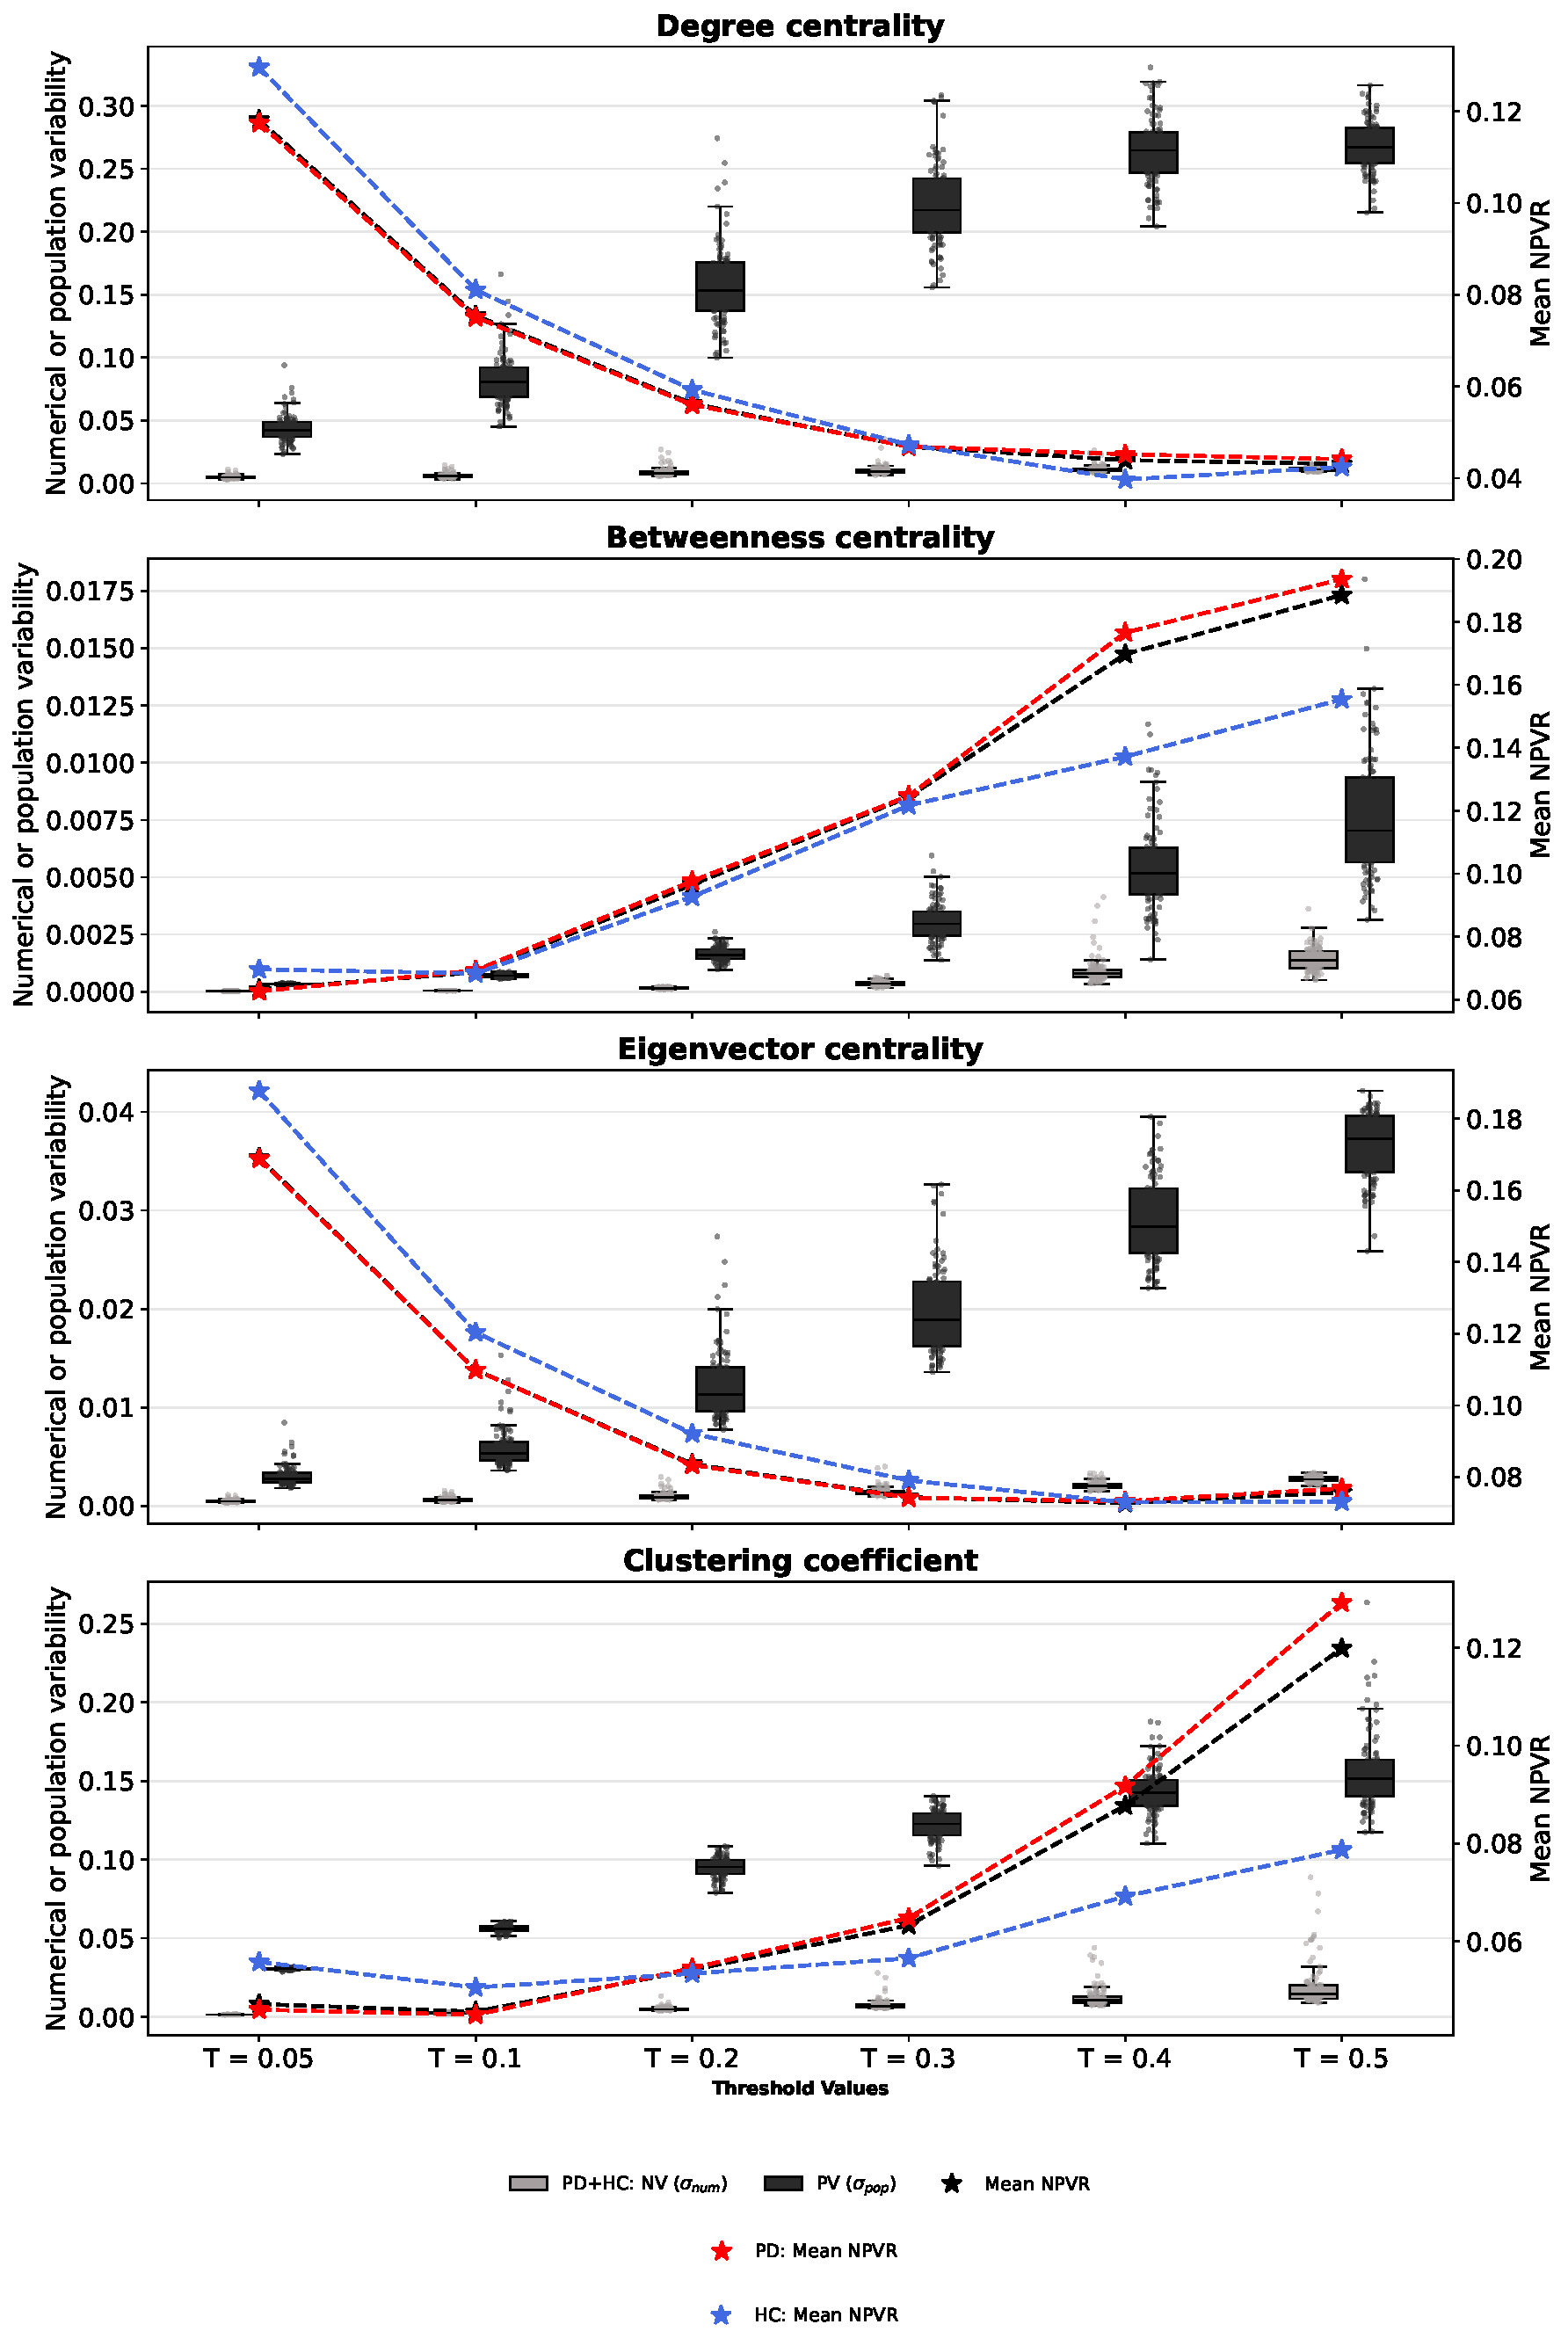
\includegraphics[width=0.80\textwidth]{Figure2.pdf}
  \caption[\npvratio{} for local graph measures]{Numerical variability, population variability, and mean \npvratio{} for local graph measures across network thresholds in the completed Phase I study. Results are shown for the pooled sample and separately for PD and healthy-control groups.}
  \label{fig:local-npvr}
\end{figure}

The region-level maps were spatially heterogeneous. At higher thresholds, clustering and betweenness in particular contained localized regions with elevated \npvratio{}. This finding matters for node-level associations because a region can be numerically sensitive even when a whole-brain average appears stable.

Confound regression changed both the magnitude and distribution of \npvratio{}. The workflow without motion-parameter regression generally had lower \npvratio{}, but this result cannot be interpreted as evidence of higher validity. Omitting nuisance regression may leave motion-related signal in the connectome. The result instead demonstrates an important thesis principle: numerical stability, data quality, and biological validity must be evaluated jointly.

\begin{figure}[htbp]
  \centering
  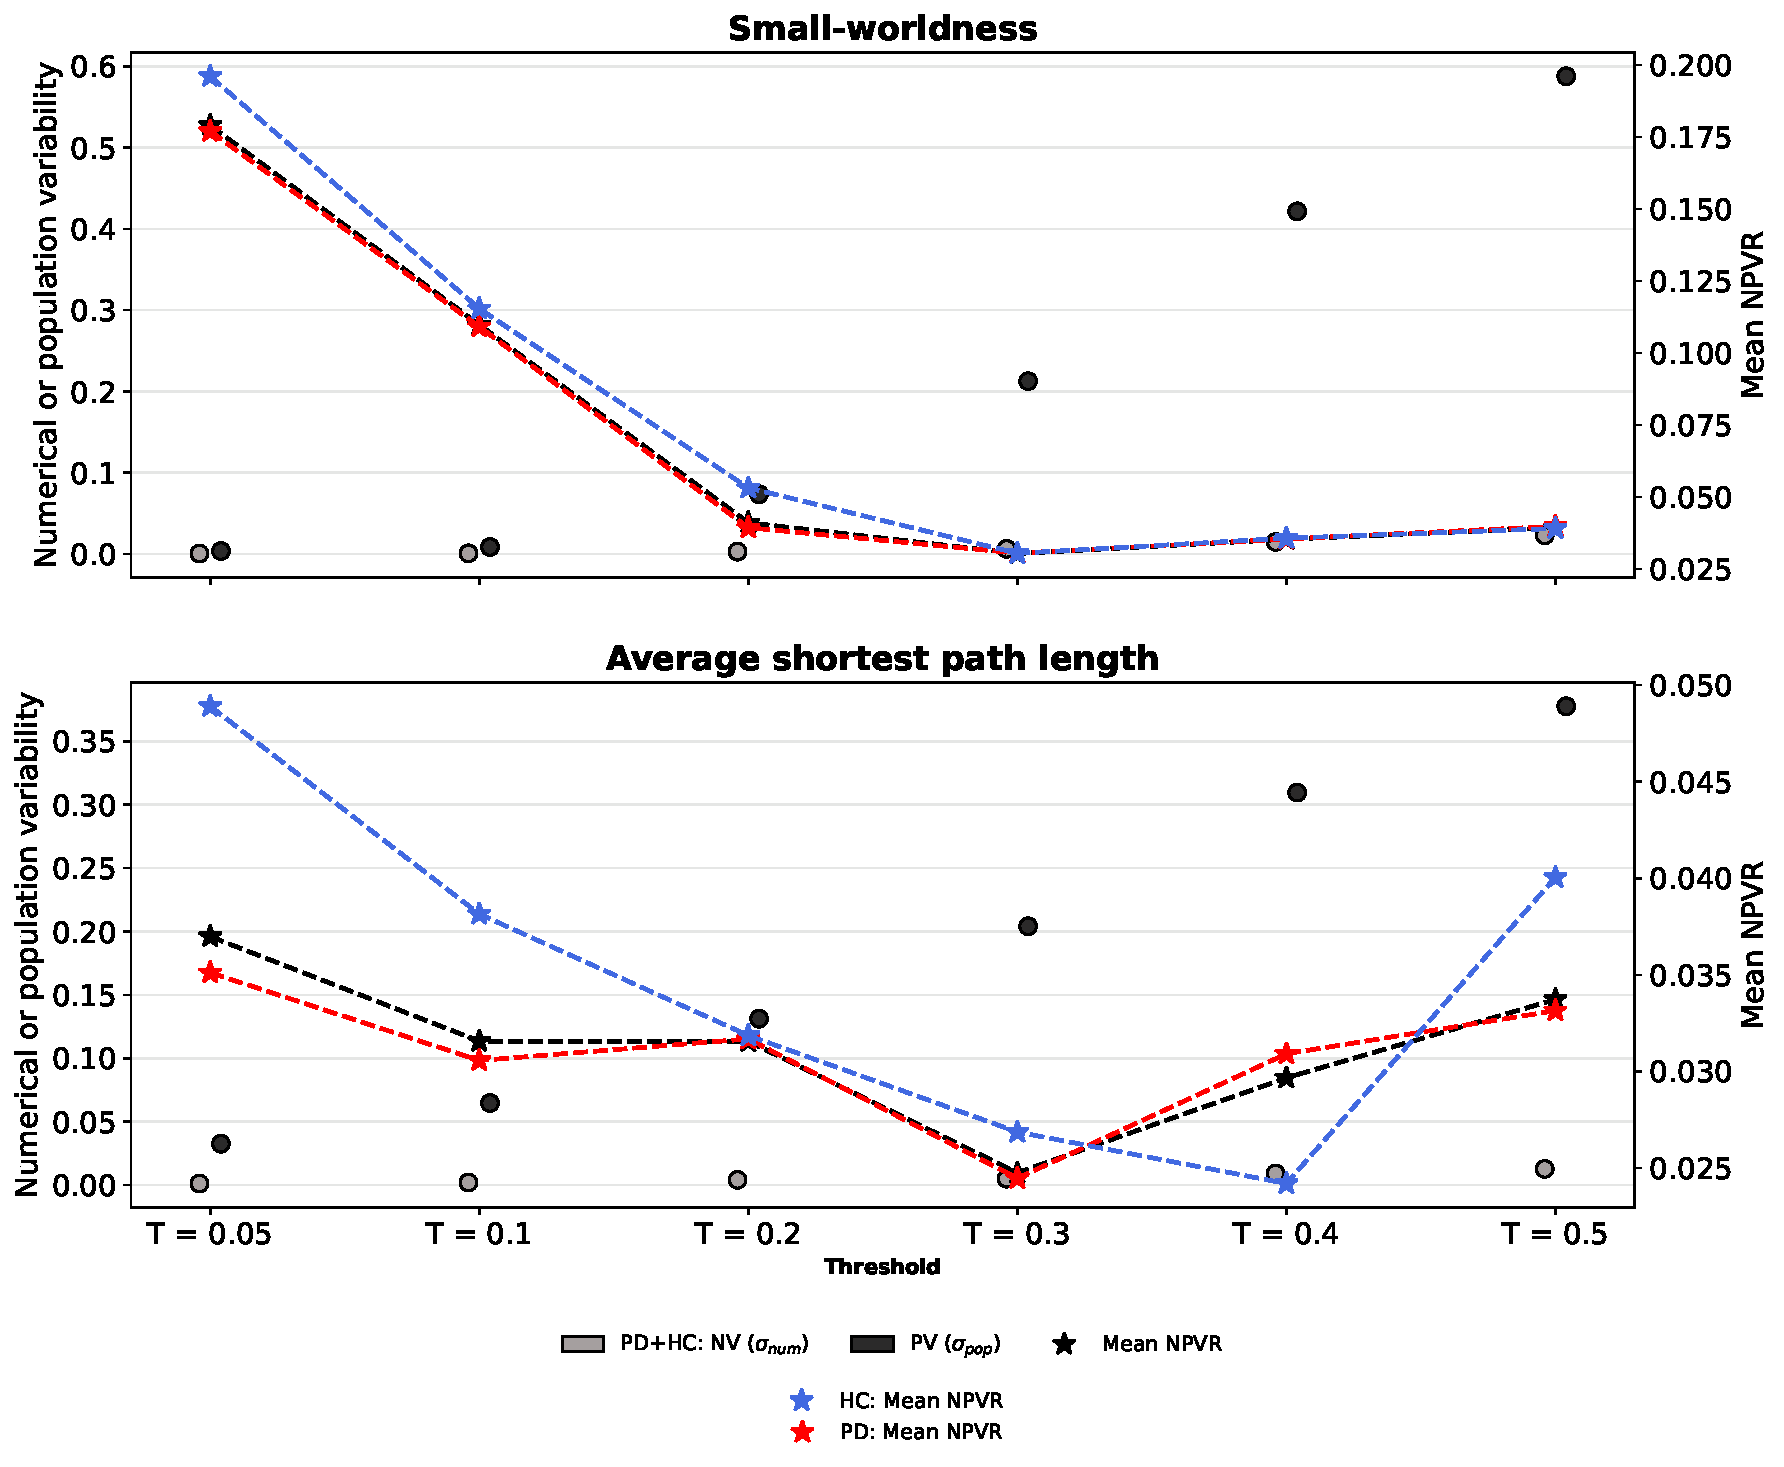
\includegraphics[width=0.98\textwidth]{Figure3.pdf}
  \caption[\npvratio{} for global graph measures]{Numerical variability, population variability, and mean \npvratio{} for small-worldness and average shortest path length across thresholds in Phase I.}
  \label{fig:global-npvr}
\end{figure}

Numerical uncertainty was most consequential for results near the significance threshold. Among 972 evaluated configurations with nominal $p$-values from 0.01 to 0.09, the pooled analysis produced a mean significance-flip probability of 17.7\%. Elevated probabilities occurred at both small and large sample sizes when the nominal result remained close to $\alpha$. Increasing sample size therefore cannot, by itself, guarantee a stable binary conclusion.

\begin{figure}[htbp]
  \centering
  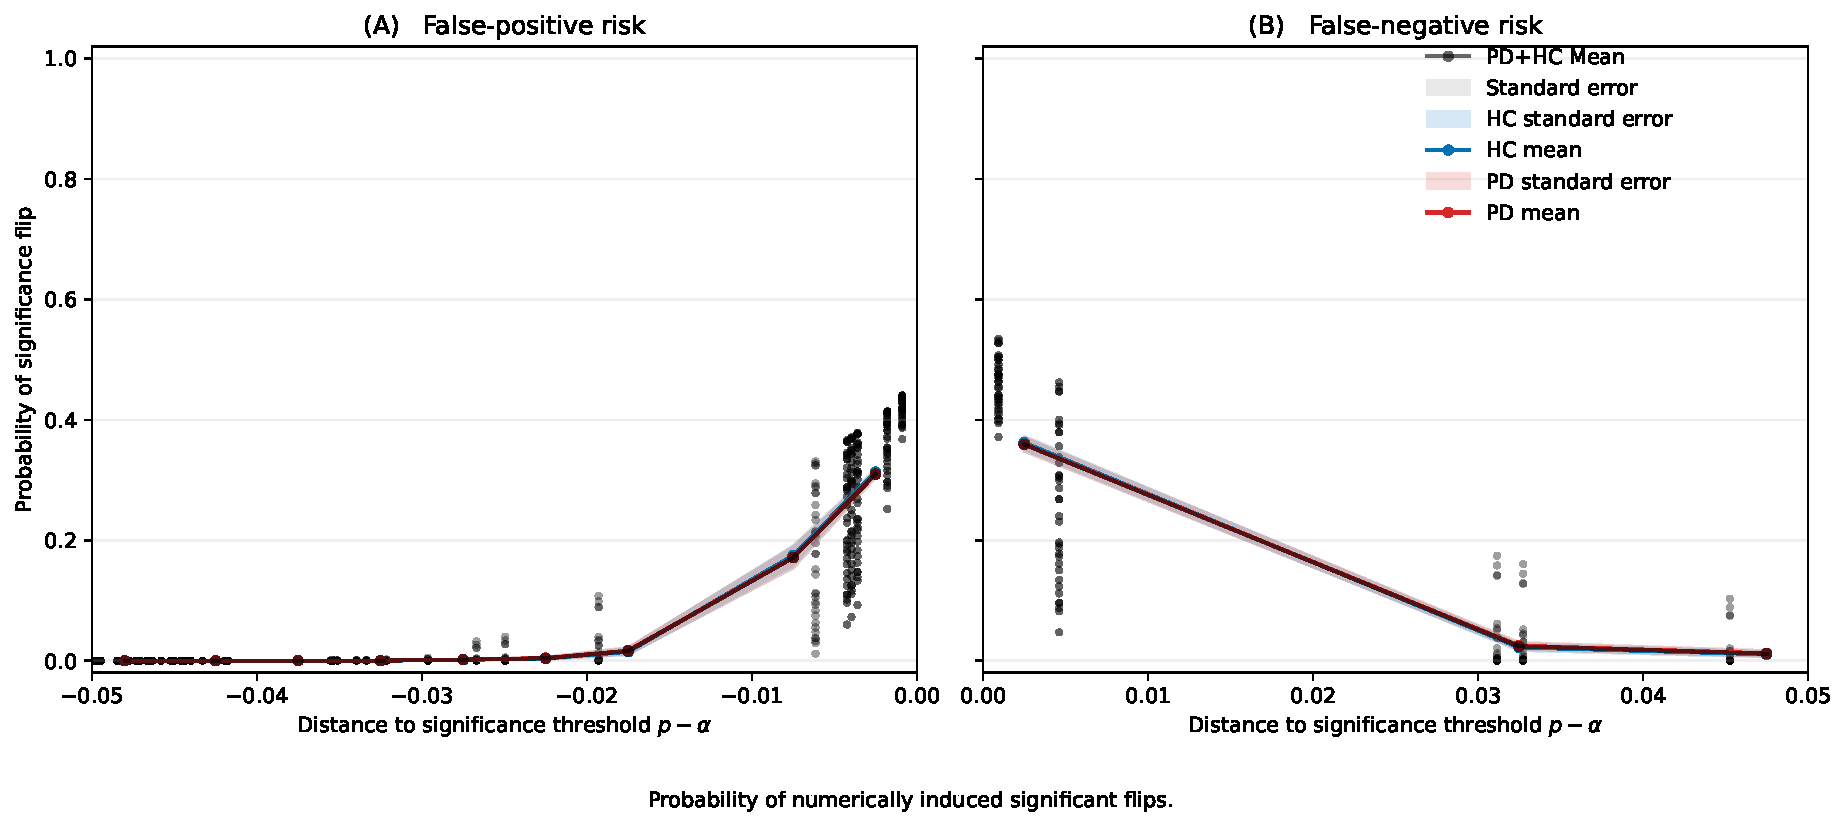
\includegraphics[width=0.98\textwidth]{Figure7.pdf}
  \caption[Probability of numerically induced significance flips]{Estimated probability of a numerically induced significance reclassification as a function of the distance between the nominal $p$-value and $\alpha=0.05$. The curves summarize configurations across graph measures, thresholds, sample sizes, and statistical tests.}
  \label{fig:flip-probability}
\end{figure}

\section{Interpretation and limitations}

Phase I establishes that low-level computational perturbations can propagate through rs-fMRI preprocessing and graph construction to quantities used for scientific inference. The magnitude is not uniform, and numerical sensitivity depends on decisions that researchers ordinarily treat as methodological choices. \npvratio{} makes the scale of this variability interpretable relative to the population, while propagation formulas expose its possible inferential consequences.

The study also defines the boundaries of the evidence. It used one principal preprocessing pipeline, one atlas resolution, absolute thresholding, cross-sectional data, and right-to-left acquisitions from PPMI. Fuzzy libmath targets mathematical-library functions and does not reproduce every possible source of infrastructure variability. Ten repetitions estimate a distribution but do not establish an exact error law. Finally, \npvratio{} depends on the population denominator and is not an accuracy measure. These limitations directly motivate the proposed future work.

\chapter{Future Work and Research Phases}
\label{chap:future-work}


\printbibliography[heading=bibintoc,title={References}]

\end{document}
